% \subsection{Relevanz des Themas}
% % Diese Arbeit adressiert diese Problematik, indem sie die Chancen und Herausforderungen von KI in der Softwareentwicklung analysiert. Ziel ist es, sowohl wissenschaftliche als auch praktische Erkenntnisse zu gewinnen, die Unternehmen und Entwicklern helfen, informierte Entscheidungen über den Einsatz von KI-gestützten Technologien zu treffen.

% % Künstliche Intelligenz (KI) hat sich in den letzten Jahren als transformative Technologie in der Softwareentwicklung etabliert. Insbesondere generative KI-Modelle wie Large Language Models (LLMs) haben das Potenzial, Entwicklungsprozesse signifikant zu verändern. Die Automatisierung von Codegenerierung, Fehleranalyse und Softwarewartung führt zu einer gesteigerten Effizienz und ermöglicht es Entwicklern, sich auf konzeptionell anspruchsvollere Aufgaben zu konzentrieren.

% % Die zunehmende Integration von KI in den Softwareentwicklungsprozess eröffnet neue Möglichkeiten, birgt jedoch auch Herausforderungen. Während einige Studien eine gesteigerte Produktivität und Codequalität durch KI-gestützte Tools belegen, gibt es gleichzeitig Bedenken hinsichtlich Sicherheitsrisiken, algorithmischer Verzerrung und langfristigen Veränderungen in der Arbeitsweise von Entwicklern. Diese Gegensätze verdeutlichen die Notwendigkeit einer fundierten wissenschaftlichen Auseinandersetzung mit den Auswirkungen von KI auf die Softwareentwicklung.

% \subsection{Motivation}
% % Die zunehmende Verbreitung künstlicher Intelligenz (KI) in der Softwareentwicklung stellt sowohl Wissenschaft als auch Praxis vor bedeutende Herausforderungen und Chancen. Unternehmen integrieren KI-gestützte Tools in ihre Entwicklungsprozesse, um Produktivität und Codequalität zu steigern, doch der langfristige Einfluss dieser Technologie auf die Arbeitsweise von Softwareentwicklern ist noch nicht vollständig erforscht.

% % Besonders relevant ist die Frage, wie sich KI-gestützte Entwicklungsumgebungen auf traditionelle Softwareentwicklungspraktiken auswirken. Während einige Forschungen darauf hindeuten, dass KI-Tools repetitive Aufgaben reduzieren und Entwicklern mehr Raum für kreative Problemlösungen geben, bestehen weiterhin Unsicherheiten hinsichtlich der Verlässlichkeit der generierten Codevorschläge und möglicher ethischer Bedenken.

Die hohe Relevanz des Themas ergibt sich aus aktuellen Entwicklungen in
Forschung und Praxis: Immer mehr Unternehmen setzen auf KI-Technologien, um
Effizienzpotenziale und Innovationsschübe zu realisieren. Während generative
KI, etwa durch automatisierte Code-Generierung oder intelligente
Projektsteuerung enorme Fortschritte und Produktivitätsgewinne verspricht,
zeigen empirische Studien zugleich ein Spannungsverhältnis zwischen den
erhofften Vorteilen und realen Risiken wie Intransparenz, Sicherheitslücken und
ethischen Verzerrungen.

Nach aktuellen Schätzungen (Stand: 2025) erreicht der Softwaremarkt in
Deutschland ein Volumen von rund 31 Milliarden US-Dollar. Entwickler:innen
verbringen im Durchschnitt bis zu 17 Stunden pro Woche mit Wartungs- und
Routineaufgaben, ein Indikator dafür, wie groß der Bedarf an Automatisierung
und Qualitätsverbesserung in der Praxis ist. Genau hier setzt die generative KI
an: Tools wie GitHub Copilot können durch automatisierte
Boilerplate-Code-Generierung oder intelligente Code-Vervollständigung nicht nur
die Produktivität erhöhen, sondern auch das Fachkräftethema teilweise
entschärfen. Laut einer von Deloitte zitierten Studie lässt sich durch
KI-basierte Coding-Tools die für Routineaufgaben benötigte Entwicklerzeit um
bis zu 50\,\% reduzieren (vgl. \cite{s_future_2024}
\cite{siebert_generative_2024}).

Ein Beleg für die zunehmende wirtschaftliche Bedeutung ist der stetige Anstieg
der Investitionen in KI-Technologien für die Softwareentwicklung in den letzten
Jahren. Abbildung~\ref{fig:ki-investitionen} veranschaulicht diese Entwicklung
und unterstreicht, wie stark Unternehmen auf innovative KI-Lösungen setzen, um
sich Wettbewerbsvorteile zu sichern.

\begin{figure}[H]
    \centering
    \vspace{1em}
    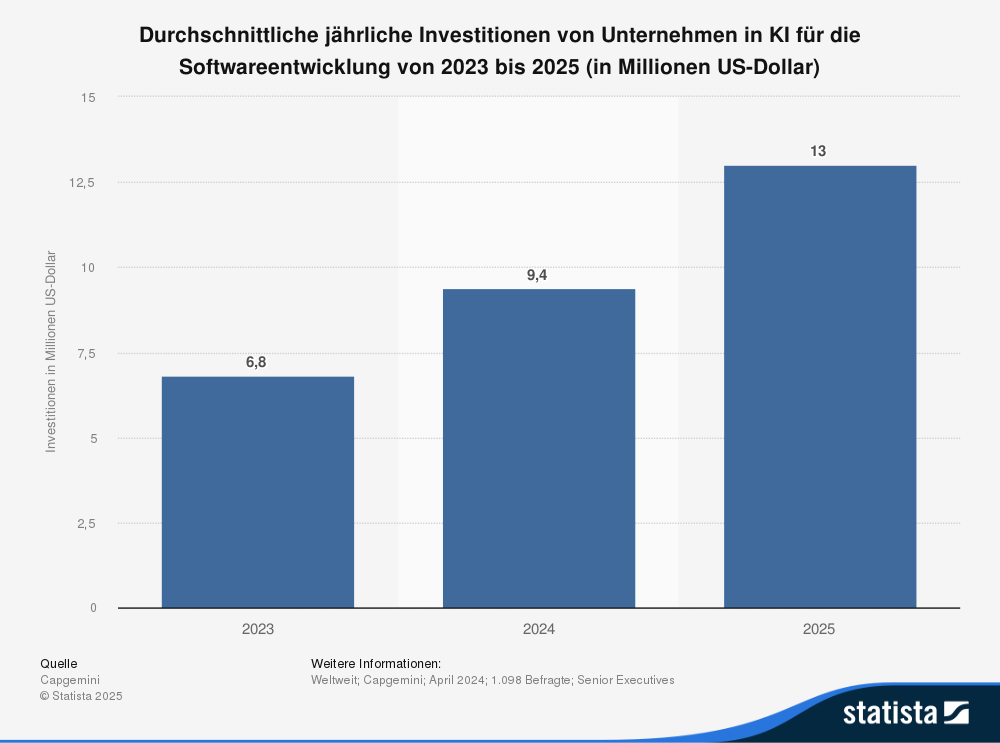
\includegraphics[width=0.7\textwidth]{images/abbildungen/statistic_id1481131_jaehrliche-investitionen-von-unternehmen-in-ki-fuer-softwareentwicklung-bis-2025.png}
    \caption{Jährliche Investitionen von Unternehmen in KI für Softwareentwicklung 2023–2025. Quelle: Capgemini~\cite{statista_ki_investitionen_2025}.}
    \label{fig:ki-investitionen}
\end{figure}

Allerdings werfen diese Entwicklungen auch kontroverse Fragen auf: In welchem
Maße verändert die zunehmende Abhängigkeit von KI-Tools die Rollen und
Kompetenzen von Softwareentwickler:innen? Wie kann sichergestellt werden, dass
durch KI-gestützte Automatisierung weiterhin qualitativ hochwertige, wartbare
und sichere Software entsteht~\cite{siebert_generative_2024}? Hinzu kommt, dass
die Softwareentwicklung durch agile Methoden wie Scrum oder Kanban bereits
stark dynamisiert ist. Die zusätzliche Integration von KI als Tool oder
„Co-Entwickler“ erhöht die Anforderungen an Prozessgestaltung, Rollenverteilung
und Qualitätsmanagement weiter.

